\documentclass{article}
\usepackage[utf8]{inputenc}
\usepackage[english, ukrainian]{babel}
\usepackage{fontsize}
\usepackage{geometry}
\usepackage{amsthm}
\usepackage{amsfonts}
\usepackage{graphicx}
\usepackage[ruled]{algorithm2e}
\usepackage{hyperref}
\usepackage{biblatex}
\usepackage{csquotes}
\usepackage{mathtools}
\usepackage{amsmath}
\usepackage{amssymb}
\usepackage{bbm}
\usepackage{tabularx}
\usepackage{xcolor}

\usepackage{tikz}
\usetikzlibrary{decorations.pathmorphing}

\usepackage{enumitem}
\usepackage{nicefrac}

\usetikzlibrary{patterns}

\usepackage{diagbox}
\usepackage{longtable}

\usepackage{float}


\usepackage{enumitem}
\usepackage{nicefrac}

\usepackage{listings}
\definecolor{codegreen}{rgb}{0,0.6,0}
\definecolor{codegray}{rgb}{0.5,0.5,0.5}
\definecolor{codepurple}{rgb}{0.58,0,0.82}
\definecolor{backcolour}{rgb}{0.95,0.95,0.92}

\lstdefinestyle{mystyle}{
    backgroundcolor=\color{backcolour},   
    commentstyle=\color{codegreen},
    keywordstyle=\color{magenta},
    numberstyle=\tiny\color{codegray},
    stringstyle=\color{codepurple},
    basicstyle=\ttfamily\footnotesize,
    breakatwhitespace=false,         
    breaklines=true,                 
    captionpos=b,                    
    keepspaces=true,                 
    numbers=left,                    
    numbersep=5pt,                  
    showspaces=false,                
    showstringspaces=false,
    showtabs=false,                  
    tabsize=2
}

\lstset{style=mystyle}
\hypersetup{colorlinks=true, linkcolor=[RGB]{255, 3, 209}, citecolor={black}}

\graphicspath{ {../Images/} }

\begin{document}
    \begin{titlepage}
        \begin{center}
        $\newline$
        \vspace{3.3cm}
        
        {\LARGE\textbf{Лабораторна робота №3\\"Реалізація алгоритму оптимізації роєм часток для пошуку глобального мінімуму функції."}}
        \vspace{10cm}
        \begin{flushright}
            \textbf{Роботу виконав:}\\Климентьєв Максим \\3-го курсу\\групи ФІ-21
        \end{flushright}
        \end{center}
    \end{titlepage}
    \newpage

    \pagenumbering{gobble}
    \tableofcontents
    \cleardoublepage
    \pagenumbering{arabic}
    \setcounter{page}{3}

    \newpage

    \section{Опис набору даних. Візуалізація прикладів з набору даних.}
    \textbf{67} внутрішніх помешкань --- \textbf{від Аеропорту до Винного погребу}

    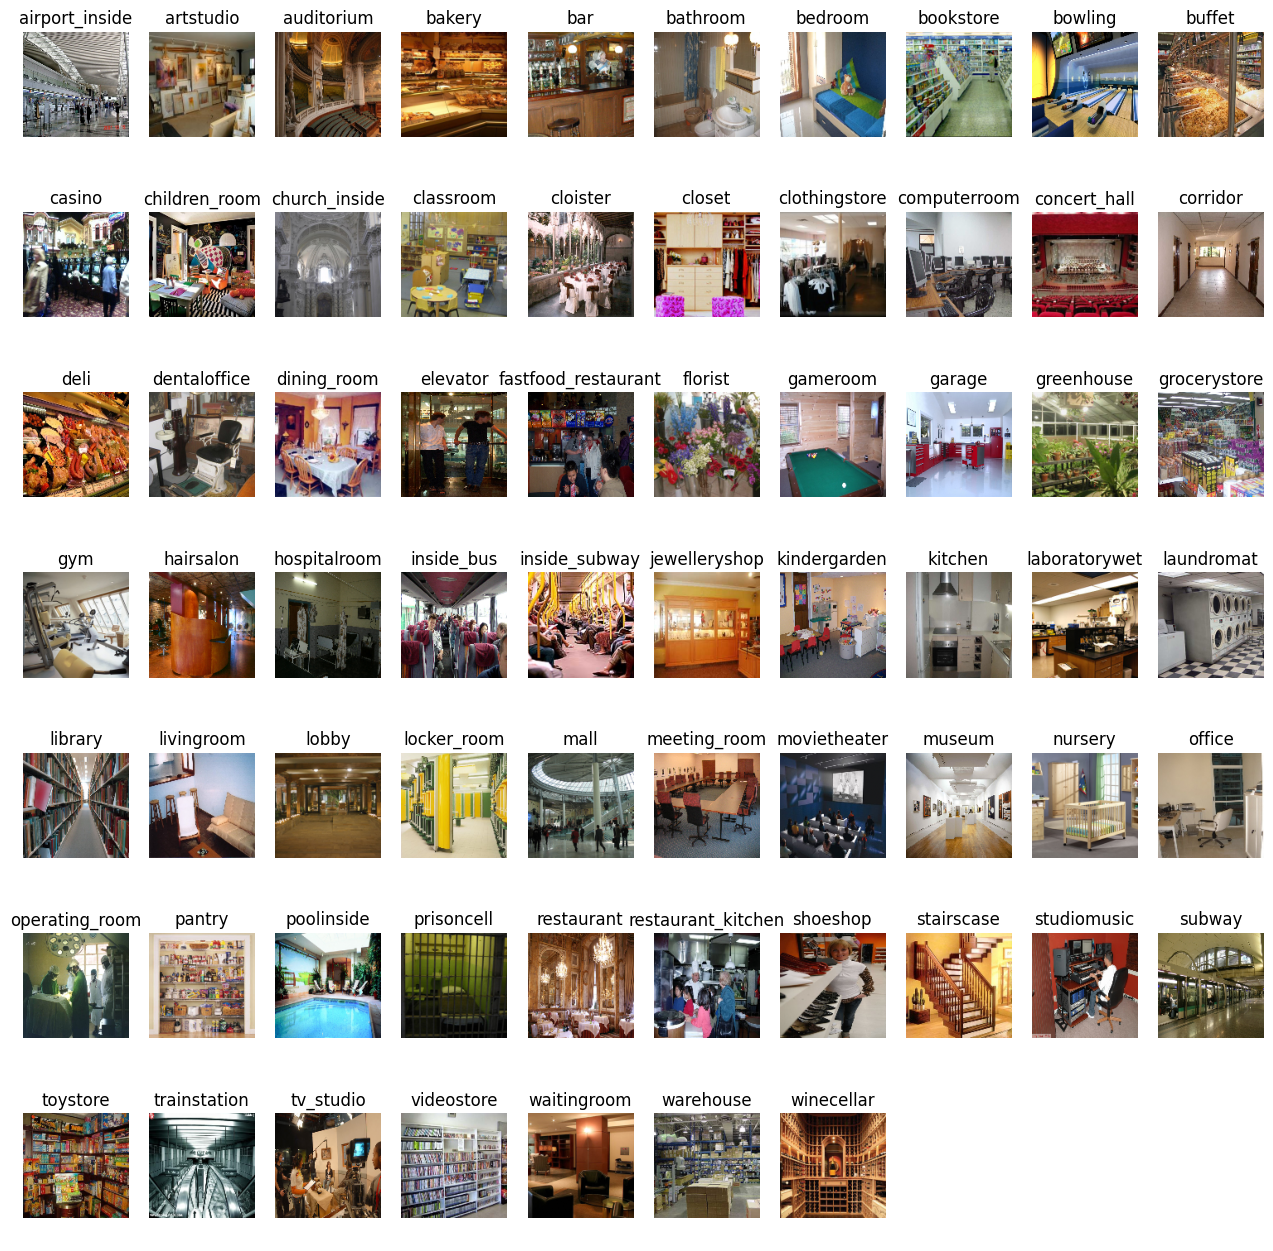
\includegraphics[width=\textwidth]{Types.png}
    \newpage

    \section{Опис базової архітектури.}
    \subsection{Архітектура нейронної мережі, кількість параметрів.}
    \begin{enumerate}
        \item 1 Conv2D 32:
            \begin{table}[h!]
                \centering
                \begin{tabular}{| c | c | c |}
                    \hline
                    Layer (type) & Output Shape & Param \\
                    \hline
                    conv2d & (None, 128, 128, 32) & 896 \\
                    \hline
                    batch\_normalization & (None, 128, 128, 32) & 128 \\
                    \hline
                    max\_pooling2d & (None, 32, 32, 32) & 0 \\
                    \hline
                    flatten & (None, 32768) & 0 \\
                    \hline
                    dense & (None, 256) & 8,388,864 \\
                    \hline
                    dropout & (None, 256) & 0 \\
                    \hline
                    dense & (None, 67) & 17,219 \\
                    \hline
                \end{tabular}
            \end{table}
        
            Total params: 8,407,107 (32.07 MB)
        
            Trainable params: 8,407,043 (32.07 MB)
        
            Non-trainable params: 64 (256.00 B)
    
        
        \item 2 Conv2D 32-32:
            \begin{table}[h!]
                \centering
                \begin{tabular}{| c | c | c |}
                    \hline
                    Layer (type) & Output Shape & Param \\
                    \hline
                    conv2d & (None, 128, 128, 32) & 896 \\
                    \hline
                    batch\_normalization & (None, 128, 128, 32) & 128 \\
                    \hline
                    max\_pooling2d & (None, 32, 32, 32) & 0 \\
                    \hline
                    conv2d & (None, 32, 32, 32) & 9,248 \\
                    \hline
                    batch\_normalization & (None, 32, 32, 32) & 128 \\
                    \hline
                    max\_pooling2d & (None, 8, 8, 32) & 0 \\
                    \hline
                    flatten & (None, 2048) & 0 \\
                    \hline
                    dense & (None, 256) & 524,544 \\
                    \hline
                    dropout & (None, 256) & 0 \\
                    \hline
                    dense & (None, 67) & 17,219 \\
                    \hline
                \end{tabular}
            \end{table}

            Total params: 552,163 (2.11 MB)

            Trainable params: 552,035 (2.11 MB)

            Non-trainable params: 128 (512.00 B)

        
        \newpage
        \item 3 Conv2D 32-32-32:
            \begin{table}[h!]
                \centering
                \begin{tabular}{| c | c | c |}
                    \hline
                    Layer (type) & Output Shape & Param \\
                    \hline
                    conv2d & (None, 128, 128, 32) & 896 \\
                    \hline
                    batch\_normalization & (None, 128, 128, 32) & 128 \\
                    \hline
                    max\_pooling2d & (None, 32, 32, 32) & 0 \\
                    \hline
                    conv2d & (None, 32, 32, 32) & 9,248 \\
                    \hline
                    batch\_normalization & (None, 32, 32, 32) & 128 \\
                    \hline
                    max\_pooling2d & (None, 8, 8, 32) & 0 \\
                    \hline
                    conv2d & (None, 8, 8, 32) & 9,248 \\
                    \hline
                    batch\_normalization & (None, 8, 8, 32) & 128 \\
                    \hline
                    max\_pooling2d & (None, 2, 2, 32) & 0 \\
                    \hline
                    flatten & (None, 128) & 0 \\
                    \hline
                    dense & (None, 256) & 33,024 \\
                    \hline
                    dropout & (None, 256) & 0 \\
                    \hline
                    dense & (None, 67) & 17,219 \\
                    \hline
                \end{tabular}
            \end{table}
        
            Total params: 70,147 (274.40 KB)
        
            Trainable params: 70,019 (273.91 KB)
        
            Non-trainable params: 128 (512.00 B)
    
        
            \item 3 Conv2D 32-64-128:
                \begin{table}[h!]
                    \centering
                    \begin{tabular}{| c | c | c |}
                        \hline
                        Layer (type) & Output Shape & Param \\
                        \hline
                        conv2d & (None, 128, 128, 32) & 896 \\
                        \hline
                        batch\_normalization & (None, 128, 128, 32) & 128 \\
                        \hline
                        max\_pooling2d & (None, 32, 32, 32) & 0 \\
                        \hline
                        conv2d & (None, 32, 32, 64) & 18,496 \\
                        \hline
                        batch\_normalization & (None, 32, 32, 64) & 256 \\
                        \hline
                        max\_pooling2d & (None, 8, 8, 64) & 0 \\
                        \hline
                        conv2d & (None, 8, 8, 128) & 73,856 \\
                        \hline
                        batch\_normalization & (None, 8, 8, 128) & 512 \\
                        \hline
                        max\_pooling2d & (None, 2, 2, 128) & 0 \\
                        \hline
                        flatten & (None, 512) & 0 \\
                        \hline
                        dense & (None, 256) & 131,328 \\
                        \hline
                        dropout & (None, 256) & 0 \\
                        \hline
                        dense & (None, 67) & 17,219 \\
                        \hline
                    \end{tabular}
                \end{table}

                Total params: 242,691 (948.01 KB)

                Trainable params: 242,243 (946.26 KB)

                Non-trainable params: 448 (1.75 KB)

        
        \newpage
        \item 6 Conv2D 32-64-128-256:
            \begin{table}[h!]
                \centering
                \begin{tabular}{| c | c | c |}
                    \hline
                    Layer (type) & Output Shape & Param \# \\
                    \hline
                    conv2d & (None, 128, 128, 32) & 896 \\
                    \hline
                    batch\_normalization & (None, 128, 128, 32) & 128 \\
                    \hline
                    max\_pooling2d & (None, 64, 64, 32) & 0 \\
                    \hline
                    conv2d & (None, 64, 64, 64) & 18,496 \\
                    \hline
                    batch\_normalization & (None, 64, 64, 64) & 256 \\
                    \hline
                    conv2d & (None, 64, 64, 64) & 36,928 \\
                    \hline
                    batch\_normalization & (None, 64, 64, 64) & 256 \\
                    \hline
                    max\_pooling2d & (None, 32, 32, 64) & 0 \\
                    \hline
                    dropout & (None, 32, 32, 64) & 0 \\
                    \hline
                    conv2d & (None, 32, 32, 128) & 73,856 \\
                    \hline
                    batch\_normalization & (None, 32, 32, 128) & 512 \\
                    \hline
                    conv2d & (None, 32, 32, 128) & 147,584 \\
                    \hline
                    batch\_normalization & (None, 32, 32, 128) & 512 \\
                    \hline
                    max\_pooling2d & (None, 8, 8, 128) & 0 \\
                    \hline
                    dropout & (None, 8, 8, 128) & 0 \\
                    \hline
                    conv2d & (None, 8, 8, 256) & 295,168 \\
                    \hline
                    batch\_normalization & (None, 8, 8, 256) & 1,024 \\
                    \hline
                    max\_pooling2d & (None, 2, 2, 256) & 0 \\
                    \hline
                    flatten & (None, 1024) & 0 \\
                    \hline
                    dense & (None, 256) & 262,400 \\
                    \hline
                    dropout & (None, 256) & 0 \\
                    \hline
                    dense & (None, 67) & 17,219 \\
                    \hline
                \end{tabular}
            \end{table}
        
            Total params: 855,235 (3.26 MB)
        
            Trainable params: 853,891 (3.26 MB)
        
            Non-trainable params: 1,344 (5.25 KB)
    
        
        \newpage

            \item 9 Conv2D 32-64-128-256:
                \begin{table}[h!]
                    \centering
                    \begin{tabular}{|c|c|c|}
                        \hline
                        Layer (type) & Output Shape & Param \# \\
                        \hline
                        conv2d & (None, 128, 128, 32) & 896 \\
                        \hline
                        batch\_normalization & (None, 128, 128, 32) & 128 \\
                        \hline
                        conv2d & (None, 128, 128, 32) & 9,248 \\
                        \hline
                        batch\_normalization & (None, 128, 128, 32) & 128 \\
                        \hline
                        max\_pooling2d & (None, 64, 64, 32) & 0 \\
                        \hline
                        conv2d & (None, 64, 64, 64) & 18,496 \\
                        \hline
                        batch\_normalization & (None, 64, 64, 64) & 256 \\
                        \hline
                        conv2d & (None, 64, 64, 64) & 36,928 \\
                        \hline
                        batch\_normalization & (None, 64, 64, 64) & 256 \\
                        \hline
                        conv2d & (None, 64, 64, 64) & 36,928 \\
                        \hline
                        batch\_normalization & (None, 64, 64, 64) & 256 \\
                        \hline
                        max\_pooling2d & (None, 32, 32, 64) & 0 \\
                        \hline
                        dropout & (None, 32, 32, 64) & 0 \\
                        \hline
                        conv2d & (None, 32, 32, 128) & 73,856 \\
                        \hline
                        batch\_normalization & (None, 32, 32, 128) & 512 \\
                        \hline
                        conv2d & (None, 32, 32, 128) & 147,584 \\
                        \hline
                        batch\_normalization & (None, 32, 32, 128) & 512 \\
                        \hline
                        conv2d & (None, 32, 32, 128) & 147,584 \\
                        \hline
                        batch\_normalization & (None, 32, 32, 128) & 512 \\
                        \hline
                        max\_pooling2d & (None, 8, 8, 128) & 0 \\
                        \hline
                        dropout & (None, 8, 8, 128) & 0 \\
                        \hline
                        conv2d & (None, 8, 8, 256) & 295,168 \\
                        \hline
                        batch\_normalization & (None, 8, 8, 256) & 1,024 \\
                        \hline
                        conv2d & (None, 8, 8, 256) & 590,080 \\
                        \hline
                        batch\_normalization & (None, 8, 8, 256) & 1,024 \\
                        \hline
                        max\_pooling2d & (None, 2, 2, 256) & 0 \\
                        \hline
                        flatten & (None, 1024) & 0 \\
                        \hline
                        dense & (None, 256) & 262,400 \\
                        \hline
                        dropout & (None, 256) & 0 \\
                        \hline
                        dense & (None, 67) & 17,219 \\
                        \hline
                    \end{tabular}
                \end{table}

                Total params: 1,640,995 (6.26 MB)

                Trainable params: 1,638,691 (6.25 MB)

                Non-trainable params: 2,304 (9.00 KB)


        
        \newpage

        \item 3 Conv2D 128-256-512:
            \begin{table}[h!]
                \centering
                \begin{tabular}{|c|c|c|}
                    \hline
                    Layer (type) & Output Shape & Param \# \\
                    \hline
                    conv2d & (None, 128, 128, 128) & 3,584 \\
                    \hline
                    batch\_normalization & (None, 128, 128, 128) & 512 \\
                    \hline
                    max\_pooling2d & (None, 32, 32, 128) & 0 \\
                    \hline
                    conv2d & (None, 32, 32, 256) & 295,168 \\
                    \hline
                    batch\_normalization & (None, 32, 32, 256) & 1,024 \\
                    \hline
                    max\_pooling2d & (None, 8, 8, 256) & 0 \\
                    \hline
                    dropout & (None, 8, 8, 256) & 0 \\
                    \hline
                    conv2d & (None, 8, 8, 512) & 1,180,160 \\
                    \hline
                    batch\_normalization & (None, 8, 8, 512) & 2,048 \\
                    \hline
                    max\_pooling2d & (None, 2, 2, 512) & 0 \\
                    \hline
                    dropout & (None, 2, 2, 512) & 0 \\
                    \hline
                    flatten & (None, 2048) & 0 \\
                    \hline
                    dense & (None, 1024) & 2,098,176 \\
                    \hline
                    dropout & (None, 1024) & 0 \\
                    \hline
                    dense & (None, 67) & 68,675 \\
                    \hline
                \end{tabular}
            \end{table}
        
            Total params: 3,649,347 (13.92 MB)
        
            Trainable params: 3,647,555 (13.91 MB)
        
            Non-trainable params: 1,792 (7.00 KB)
    
\end{enumerate}

\newpage
    \subsection{Точність класифікації.}

    \foreach \x in {1,2,...,7}
    {
        \begin{figure}[H]
            \centering
            \includegraphics[width=0.5\linewidth]{accuracy_\x.png}
            \caption{\x}
        \end{figure}
    }

    \newpage
    \subsection{Візуалізація функцій втрат (тестовий та тренінговий набір).}

    \foreach \x in {1,2,...,7}
    {
        \begin{figure}[H]
            \centering
            \includegraphics[width=0.5\linewidth]{loss_\x.png}
            \caption{\x}
        \end{figure}
    }
    \newpage

    % \subsection{Параметри точності класифікації.}

    \section{Опис експериментів.}
    \subsection{Які зміни було внесено.}
    \begin{itemize}
        \item Базова версія - 1 Conv2D 32
        \item Run №2 - 2 Conv2D 32-32

        \item Run №3 - 3 Conv2D 32-32-32
        \item Run №4 - 3 Conv2D 32-64-128

        \item Run №5 - 6 Conv2D 32-64-128-256
        \item Run №6 - 9 Conv2D 32-64-128-256

        \item Run №7 - 3 Conv2D 128-256-512

    \end{itemize}

    \subsection{Висновки: як це вплинуло на результат, процес тренування, ...}
        Більше Conv2D дає більше точності, але, скоріше за все, вище 50\% не отримати, треба ще використовувати щось окрім Conv2D, наприклад, збільшити розмір зображення.

    \section{Результати порівняння.}
    \begin{table}[h!]
        \centering
        \begin{tabular}{| c | c | c | c | c | c | c |}
            \hline
            Опис & Conv2D & Top2 & Acc & Loss & Epoch & Tr. Time \\
            \hline
            Базова & 1 & 18 & 10 & 396 & 40 & 87 \\
            \hline
            Run №2 & 2 & 38 & 25 & 363 & 40 & 77 \\
            \hline
            Run №3 & 3 & 46 & 31 & 299 & 40 & 74 \\
            \hline
            Run №4 & 3 & 47 & 33 & 363 & 40 & 80 \\
            \hline
            Run №5 & 6 & 54 & 41 & 336 & 100 & 275 \\
            \hline
            Run №6 & 9 & 52 & 39 & 419 & 70 & 468 \\
            \hline
            Run №7 & 3 & 51 & 38 & 476 & 70 & 475 \\
            \hline
            Best №7 & 3 & 58 & 45 & 347 & 63 & 475 \\
            \hline
        \end{tabular}
    \end{table}

    \section{Висновки.}
    Найкраще, що вдалося отримати простою моделлю - 45\% точності, але з досить великими втратами.

\end{document}